\documentclass[a4paper, 12.5pt]{scrartcl}
\usepackage{german}
\usepackage[utf8]{inputenc}
\usepackage{graphicx}
\usepackage{amsmath}
\graphicspath{{./Figures/}}
\usepackage{hyperref}


\begin{document}


\begin{titlepage}
\author{Justin Sprenger (s0556255), 
Lukas Wagner (s0556753)} 
\title{Android Chat Applikation auf Basis des SPIRIT1} 
\date{\today} 
\maketitle
\end{titlepage}

\tableofcontents
\newpage
\section{Einleitung}
\subsection{Zusammenfassung}

Ziel des Projekts ist die Entwicklung und Implementierung einer Android-Applikation, die den ad-hoc-Austausch von Daten zwischen mehreren Geräten über den Transceiver SPIRIT1 des Herstellers STMicroelectronics ermöglicht.  Der Funktionalitätsumfang der Applikation umfasst grundlegende Funktionen, Chatnachrichten können versendet und empfangen werden. 
Schlüsselwörter: low data rate, low energy Transceiver; RF module; Android

\subsection{Mitwirkende}

An dem Projekt haben mitgewirkt: Herr Justin Sprenger und Herr Lukas Wagner. Zu Beginn des Projektes wurden unabhängig voneinander verschiedene Herangehensweisen untersucht (s. 4.a. Lösungsansätze). Nach der Probierphase haben sich beide auf eine Vorgehensweise geeinigt und von da an gemeinsam die Anwendung implementiert, getestet, sowie Recherchen durchgeführt (s. Abschnitt 4.b).
\section{Grundlagen}

\subsection{Kurzbeschreibung des STEVAL-SP1ML868}

Der STEVAL-SP1ML868, im Folgenden STEVAL oder Dongle genannt, hat die Funktion den SPIRIT1 RF Transceiver testbar zu machen, der Dongle als Evaluation Tool ist an sich kein Produkt für den Markt. Die Ausstattung umfasst einen USB Anschluss, sodass über einen PC die Energieversorgung sowie der Zugriff auf das RF Modul gewährleistet wird. Mittels AT Befehle wird das RF Modul über den STEVAL angesprochen. AT Befehle können über verschiedene Terminalprogramme getestet werden. In dem Beispiel des Herstellers und auch in der frühen Testphase diesen Projektes wurde das Programm Hyperterminal verwendet.
AT Befehle:	Mit der Eingabe “+++” gelangt der Nutzer in den Command Mode und kann AT Befehle ausführen. Der AT Befehl “at/s” ruft die Settings auf (s. Abb.). Ein Setting wird mit der Sequenz “ats<Setting Code>=<Setting Wert>” verändert und anschließend mit “at/c” gespeichert. Zum Senden und Empfangen wechselt man mit “ato” vom Command Mode in den standardmäßigen Operation Mode.
\begin{figure}[h]
	\centering
	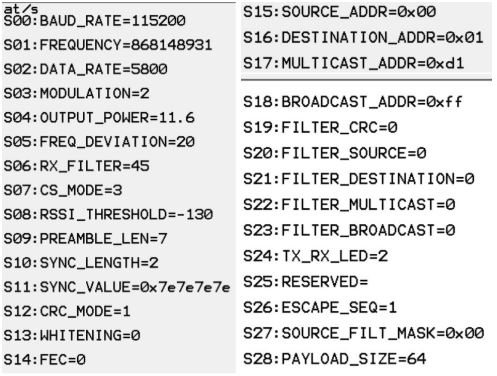
\includegraphics[scale=1.0]{at.jpg}
	\caption{AT/S - Befehle}
	\label{img:ats}
\end{figure}
\newpage
\subsection{Kurzbeschreibung des SPIRIT1} 

Der SPIRIT1 Transceiver ist ein low data rate, low power, sub 1GHz RF Transceiver. Die Datenübertragungsrate kann eingestellt werden zwischen 1 und 500 kbps, der Energieverbrauch liegt bei einem Leistungspegel von 11 dBm im Bereich 9 mA beim Empfangen und 21 mA beim Senden (vgl. Datasheet SPIRIT1 S. 1). Die Frequenzbereiche reichen von 150 MHz bis 956 MHz. 

\section{Implementierung der Anwendung}

\subsection{Lösungsansätze}

Zunächst wurde versucht auf die neu erschienene Android Things API zurück zu greifen, jedoch stellte sich heraus, dass nur Android Geräten mit dem neuesten Android Operating System 8.1 die API nutzen können. Die Verbreitung von Android 8.1 ist zu diesem Zeitpunkt limitiert auf einzelne Geräte der Pixel Baureihe und Nexus Smartphones und kommt daher für dieses Projekt nicht in Frage. Desweiteren wurde mit der Android Library “android.hardware.usb” gearbeitet. Diese Library bietet die Möglichkeit über die USB-Schnittstelle des Smartphones seriell Daten zu übertragen. Die UART-Einstellungen (Baudrate, Parität, Stopbit, Flussrichtung, Databit) werden im Quellcode als Hexcode angegeben. Es kann synchron oder asynchron übertragen werden. In beiden Fällen werden zunächst die Endpoints für Senden und Empfangen aus dem Dongle ausgelesen. Eine Implementierung aller notwendigen Methoden hätte den Rahmen des Projektes überschritten, um den Anforderungen der Aufgabenstellung gerecht zu werden, wurde eine open Source API ausgesucht, welche die android.hardware.usb Library implementiert.

\subsection{Umsetzung mit der usb-serial-for-Android Library}

Die usb-serial-for-Android Library stellt verschiedene Treiber für serielle Datenübertragung zur Verfügung. Für den STEVAL ist der CP21xxSerialPort Treiber geeignet.

\subsubsection{Empfangen}

Bei der Übertragung werden durchgängig Signale aufgefangen, die nicht für die Chat Applikation bestimmt sind. Solche Signale müssen herausgefiltert werden um den Chat lesbar zu halten. Eine Filterung nach Mustern in den Signalen kommt nicht in Frage, da die Signale, gleich unseren Nachrichten, aus Buchstaben, Zahlen, auch Sonderzeichen bestehen. Stattdessen ist der Ansatz einen Key mitzusenden praktikabel. Die App kann die autorisierten Nachrichten an einer einfachen Ziffernsequenz erkennen und filtert alle anderen Nachrichten aus. Der Key muss aus einem mehrfach wiederkehrenden Zeichen bestehen um die Abfrage übertragunssicher zu gestalten und auch nach dem Verlust einzelner Zeichen noch akzeptiert zu werden. Die Chat Applikation hat den Key “\_\_\_\_\_” implementiert. Der Key wird auf zwei zusammenhängende Underscores geprüft. Letztendlich wird auch der Key ausgefiltert um die Lesbarkeit zu steigern.
\begin{figure}[h]
	\centering
	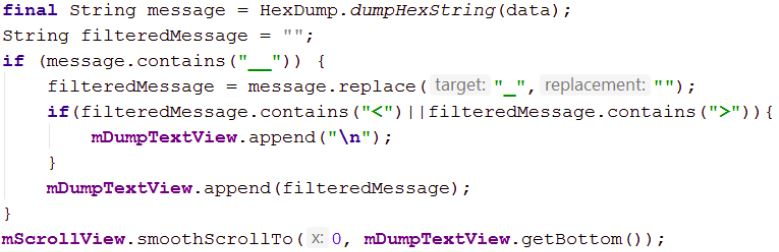
\includegraphics[scale=1.0]{read.jpg}
	\caption{Code-Read-Methode}
	\label{img:read}
\end{figure}
\newpage
\subsubsection{Senden}

Die Payload des RF Moduls ist begrenzt auf 64 bit, möchte der User eine längere Nachricht schreiben, wird diese bitweise unterteilt (s. Abb.) und in mehreren Teilen gesendet. Bei jeder dieser Teilnachrichten wird zur Autorisierung der Key erneut als Präfix gesetzt. Damit der Chat nutzerfreundlich ist und die Kommunikationspartner trotz Broadcast Sendeverhalten die Übersicht wahren, wird der Username mit der Nachricht übermittelt. Dem Nutzer der Applikation werden sowohl die eigenen Nachrichten angezeigt, als auch die Nachrichten der Chatpartner, jeweils mit Nutzernamen versehen.
\begin{figure}[h]
	\centering
	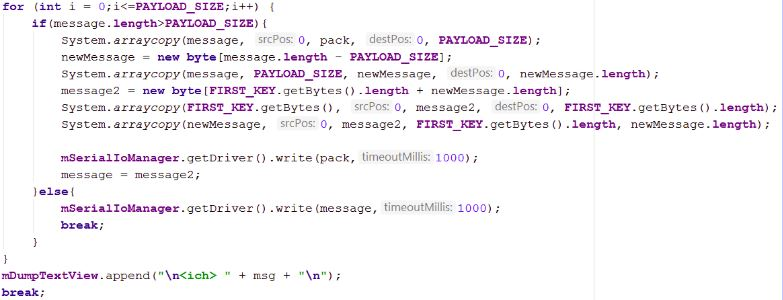
\includegraphics[scale=1.0]{write.jpg}
	\caption{Code-Write-Methode}
	\label{img:write}
\end{figure}
\newpage
\subsubsection{Settings}

Zunächst wurden die Standardeinstellungen aus dem Quick User Manual übernommen. Die Baudrate liegt bei 11 5200 Bd, das Paritätsbit wird nicht gesetzt, Stopbit bei einem Bit, die Frequenz bei 868 MHz, die RSSI threshold bei -130 und Flusskontrolle ausgeschaltet. Für die Optimierung der Applikation sind einige Register des RF Moduls über AT Befehle angepasst worden. Der CS Mode wurde auf Modus 0 eingestellt. Somit wird der RSSI threshold als statische Schwelle für die Kenntnisnahme eines Signals verwendet. Signale mit einer Stärke über dem RSSI threshold werden empfangen, 3 dB darunter nicht (vgl. SPIRIT1 Datasheet S. 72). Der CRC Mode wurde mit Modus 1 auf ein kurzes Polynom mit 8 bit Länge gesetzt (vgl. SPIRIT1 Datasheet S.61). Die Payload size wurde von 8 bit auf 64 bit erhöht um den Bitbedarf für die Mitsendung des Keys und des Usernamens möglichst gering zu halten.

\subsection{Probleme}

Ein Problem, welches das Projekt durchgehend begleitet hat, war das aufwendige Testen der Software. Da der Emulator von Android Studio nicht mit dem Dongle kommunizieren kann, musste für jeden Testdurchgang die Applikation auf ein bis zwei Android Geräte gespielt und an die Evaluation Boards angeschlossen werden. Jeder noch so kleine Test hat mehrere Minuten in Anspruch genommen.
Die Wahl des Keys mit der Zeichenfolge “+++++” hat sich über einen langen Zeitraum als kritisches Hindernis herausgestellt, da der Key sich mit dem AT Command für den Command Mode des Dongle überschneidet und ein Senden, bzw. Empfangen unmöglich macht. Die erste Nachricht wurde gesendet und empfangen, danach hat die Applikation nicht mehr funktioniert. 
Ein weitere Hürde ist die mangelhaft Übertragungsgenauigkeit der RF Module. Am Anfang kamen lediglich einzelne Buchstaben korrekt an, nach der Konfigurierung der Register verbesserte sich die Übertragung und die Nachrichten wurden lesbar. Doch selbst zum Abschluss des Projektes ist die Zahl der Übertragungsfehler unbefriedigend hoch.


\section{Reichweitenmessung}
Indoor ca. 80 m
\newline
Outdoor ca. 200 m

\newpage

\section{Literaturverzeichnis}
\begin{thebibliography}{1}

\bibitem{STMicroelectronics (2016). SPIRIT1 Datasheet} STMicroelectronics (2016). SPIRIT1 Datasheet {\em https://www.st.com/content/st_com/en/products/wireless-connectivity/sub-1ghz-rf/spirit1.html}

\bibitem{STMIcroelectronics (2016). UM1889 User manual}STMIcroelectronics (2016). UM1889 User manual {\em https://www.st.com/en/evaluation-tools/steval-sp1ml868.html}

\bibitem{STMicroelectronics (2015). STEVAL_SP1ML868 Datasheet}STMicroelectronics (2015). STEVAL_SP1ML868 Datasheet {\em https://www.st.com/en/evaluation-tools/steval-sp1ml868.html}

\end{thebibliography}

\section{Anhang}

\end{document}